\documentclass[12pt]{book}

\usepackage{pdfpages}
\usepackage{hyperref}
\usepackage{xeCJK}
\usepackage{xcolor}
\usepackage[top=2cm, bottom=2cm, left=4cm, right=3cm]{geometry}
\pagestyle{empty}

\tolerance=1
\emergencystretch=\maxdimen
\hyphenpenalty=10000
\hbadness=10000

\begin{document}
	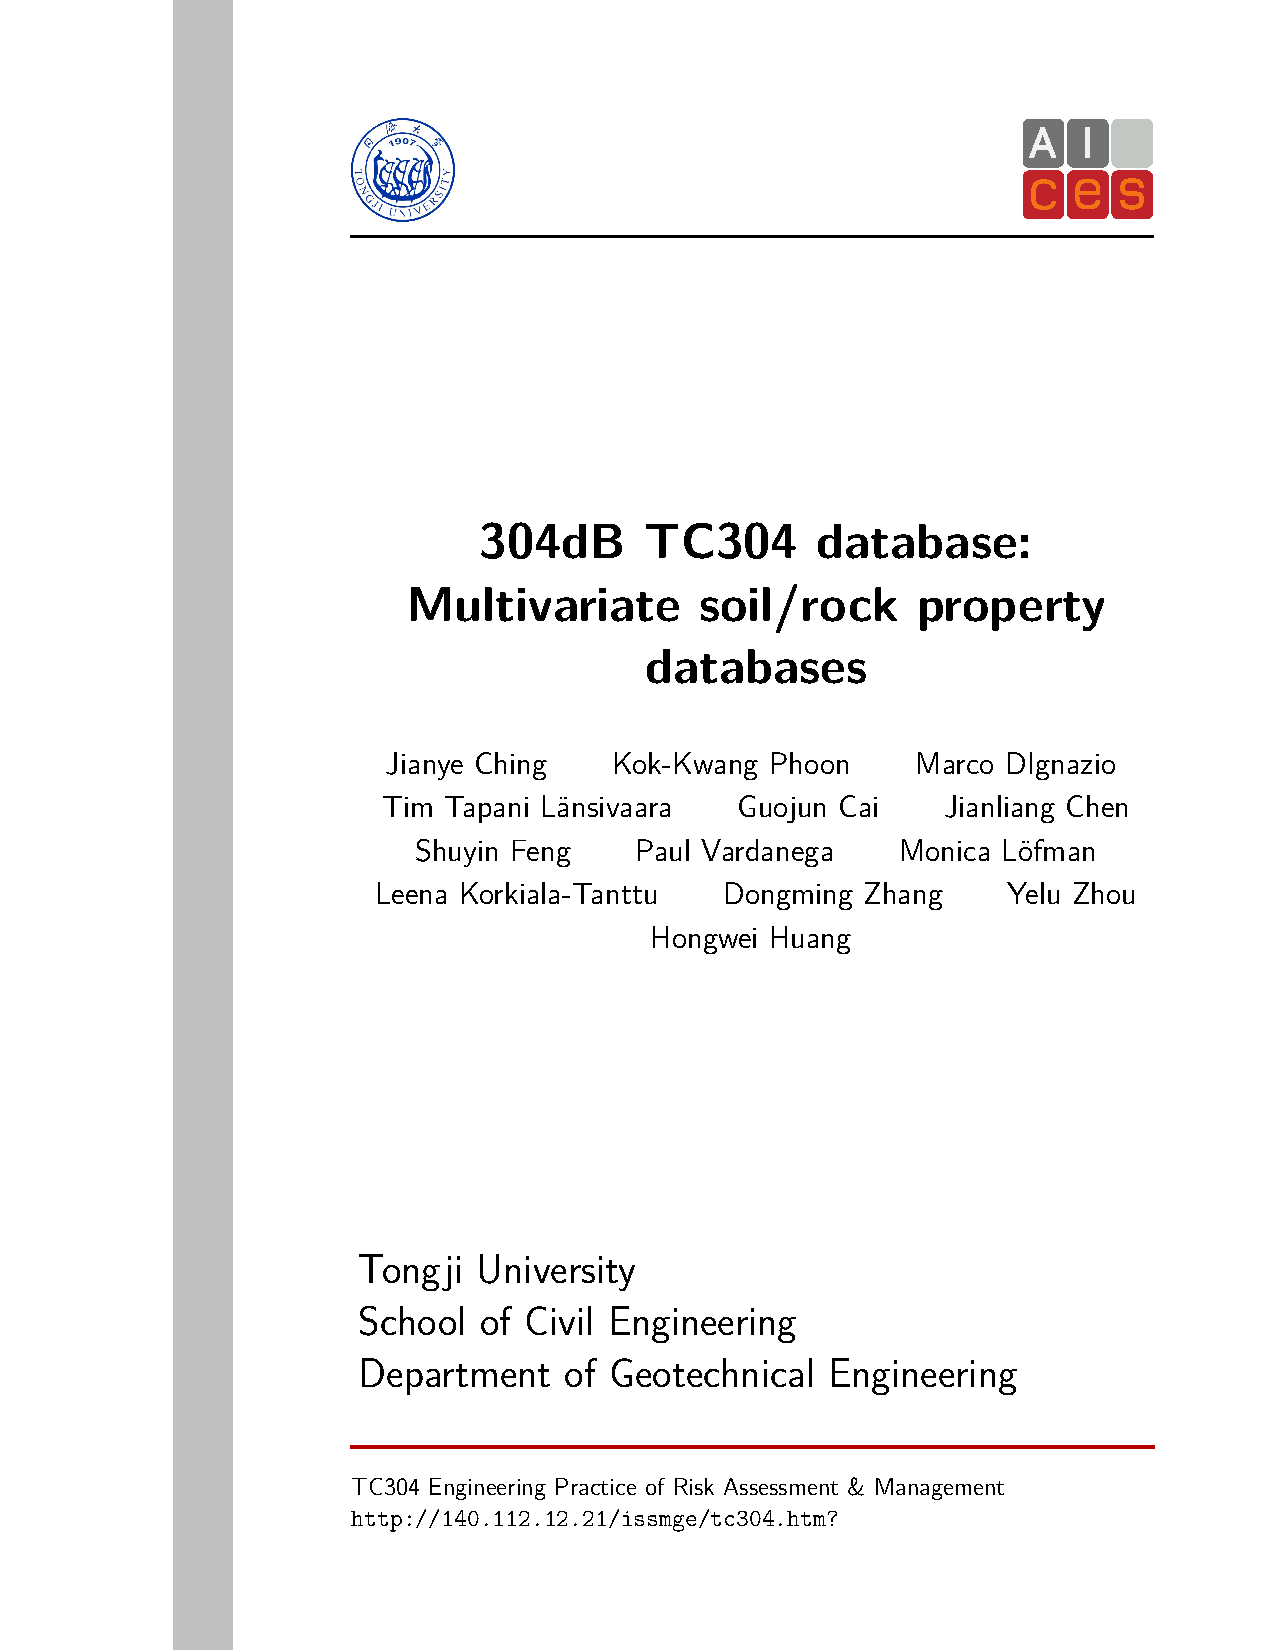
\includepdf{Cover.pdf}
	\cleardoublepage

	\begin{center}
		\bfseries\centering\Large Table of Contents
	\end{center}
	\par

	\begin{itemize}
		\item[\textcolor{red}{CLAY/5/345}] \textcolor{blue}{Ching2012}-Modeling parameters of structured clays as a multivariate normal distribution \hfill\textcolor{red}{\pageref{bib:1}}
		\item[\textcolor{red}{CLAY/6/535}] \textcolor{blue}{Ching2014}-Modeling piezocone cone penetration (CPTU) parameters of clays as a multivariate normal distribution \hfill\textcolor{red}{\pageref{bib:2}}
		\item[\textcolor{red}{CLAY10/7490}] \textcolor{blue}{Ching2014}-Transformations and correlations among some clay parameters - the global database \hfill\textcolor{red}{\pageref{bib:3}}
		\item[\textcolor{red}{CLAY10/7490}] \textcolor{blue}{Ching2014}-Correlations among some clay parameters - the multivariate distribution \hfill\textcolor{red}{\pageref{bib:4}}
		\item[\textcolor{red}{F-CLAY/7/216}] \textcolor{blue}{D’Ignazio2016}-Correlations for undrained shear strength of Finnish soft clays \hfill\textcolor{red}{\pageref{bib:5}}
		\item[\textcolor{red}{S-CLAY/7/168}] \textcolor{blue}{D’Ignazio2016}-Correlations for undrained shear strength of Finnish soft clays \hfill\textcolor{red}{\pageref{bib:6}}
		\item[\textcolor{red}{J-CLAY/5/124}] \textcolor{blue}{Liu2016}-Multivariate correlation among resilient modulus and cone penetration test parameters of cohesive subgrade soils \hfill\textcolor{red}{\pageref{bib:7}}
		\item[\textcolor{red}{SAND/7/2794}] \textcolor{blue}{Ching2017}-Transformation models for effective friction angle and relative density calibrated based on generic database of coarse-grained soils \hfill\textcolor{red}{\pageref{bib:8}}
		\item[\textcolor{red}{ROCK/9/4069}] \textcolor{blue}{Ching2018}-Generic transformation models for some intact rock properties \hfill\textcolor{red}{\pageref{bib:9}}
		\item[\textcolor{red}{FG-KSAT/6/1358}] \textcolor{blue}{Feng2019a}-A database of saturated hydraulic conductivity of fine-grained soils- probability density functions \hfill\textcolor{red}{\pageref{bib:10}}
		\item[\textcolor{red}{FG-KSAT/6/1358}] \textcolor{blue}{Feng2019b}-Full AccessCorrelation of the hydraulic conductivity of fine-grained soils with water content ratio using a database \hfill\textcolor{red}{\pageref{bib:11}}
		\item[\textcolor{red}{ROCKMass/9/5876}] \textcolor{blue}{Ching2020}-Quasi-site-specific prediction for deformation modulus of rock mass \hfill\textcolor{red}{\pageref{bib:12}}
		\item[\textcolor{red}{SH-CLAY/11/4051}] \textcolor{blue}{Zhang2020}-Multivariate probability distribution of shanghai clay properties \hfill\textcolor{red}{\pageref{bib:13}}
		\item[\textcolor{red}{14}] Ching2020-Quasi-site-specific prediction for deformation modulus of rock mass \hfill\textcolor{red}{\pageref{bib:14}}
		\item[\textcolor{red}{14}] Liu2016-Multivariate correlation among resilient modulus and cone penetration test parameters of cohesive subgrade soils \hfill\textcolor{red}{\pageref{bib:15}}
	\end{itemize}
	\cleardoublepage

	\includepdfset{pagecommand={\thispagestyle{headings}}}
	\setcounter{page}{1}

	\label{bib:1}
	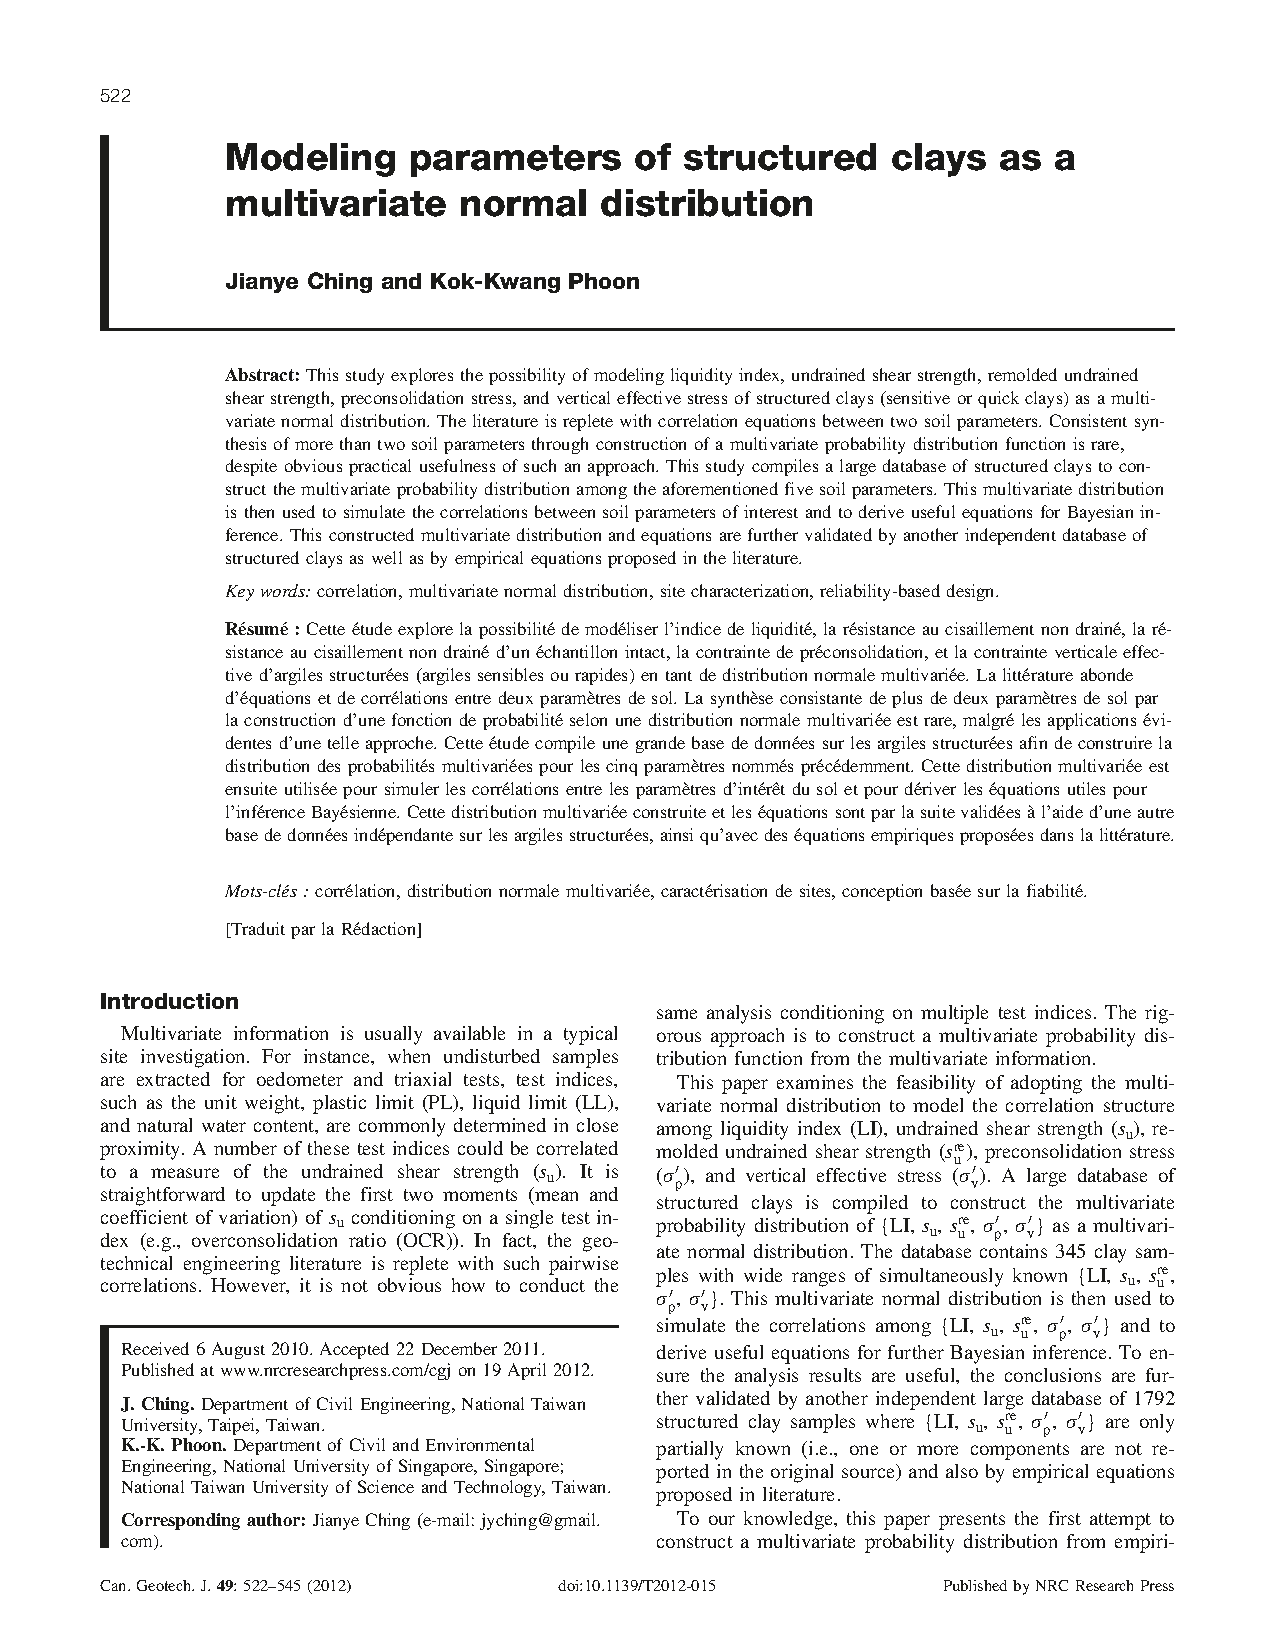
\includepdf[pages=1-last]{PDFs/Ching2012-Modeling parameters of structured clays as a multivariate normal distribution.pdf}
	\label{bib:2}
	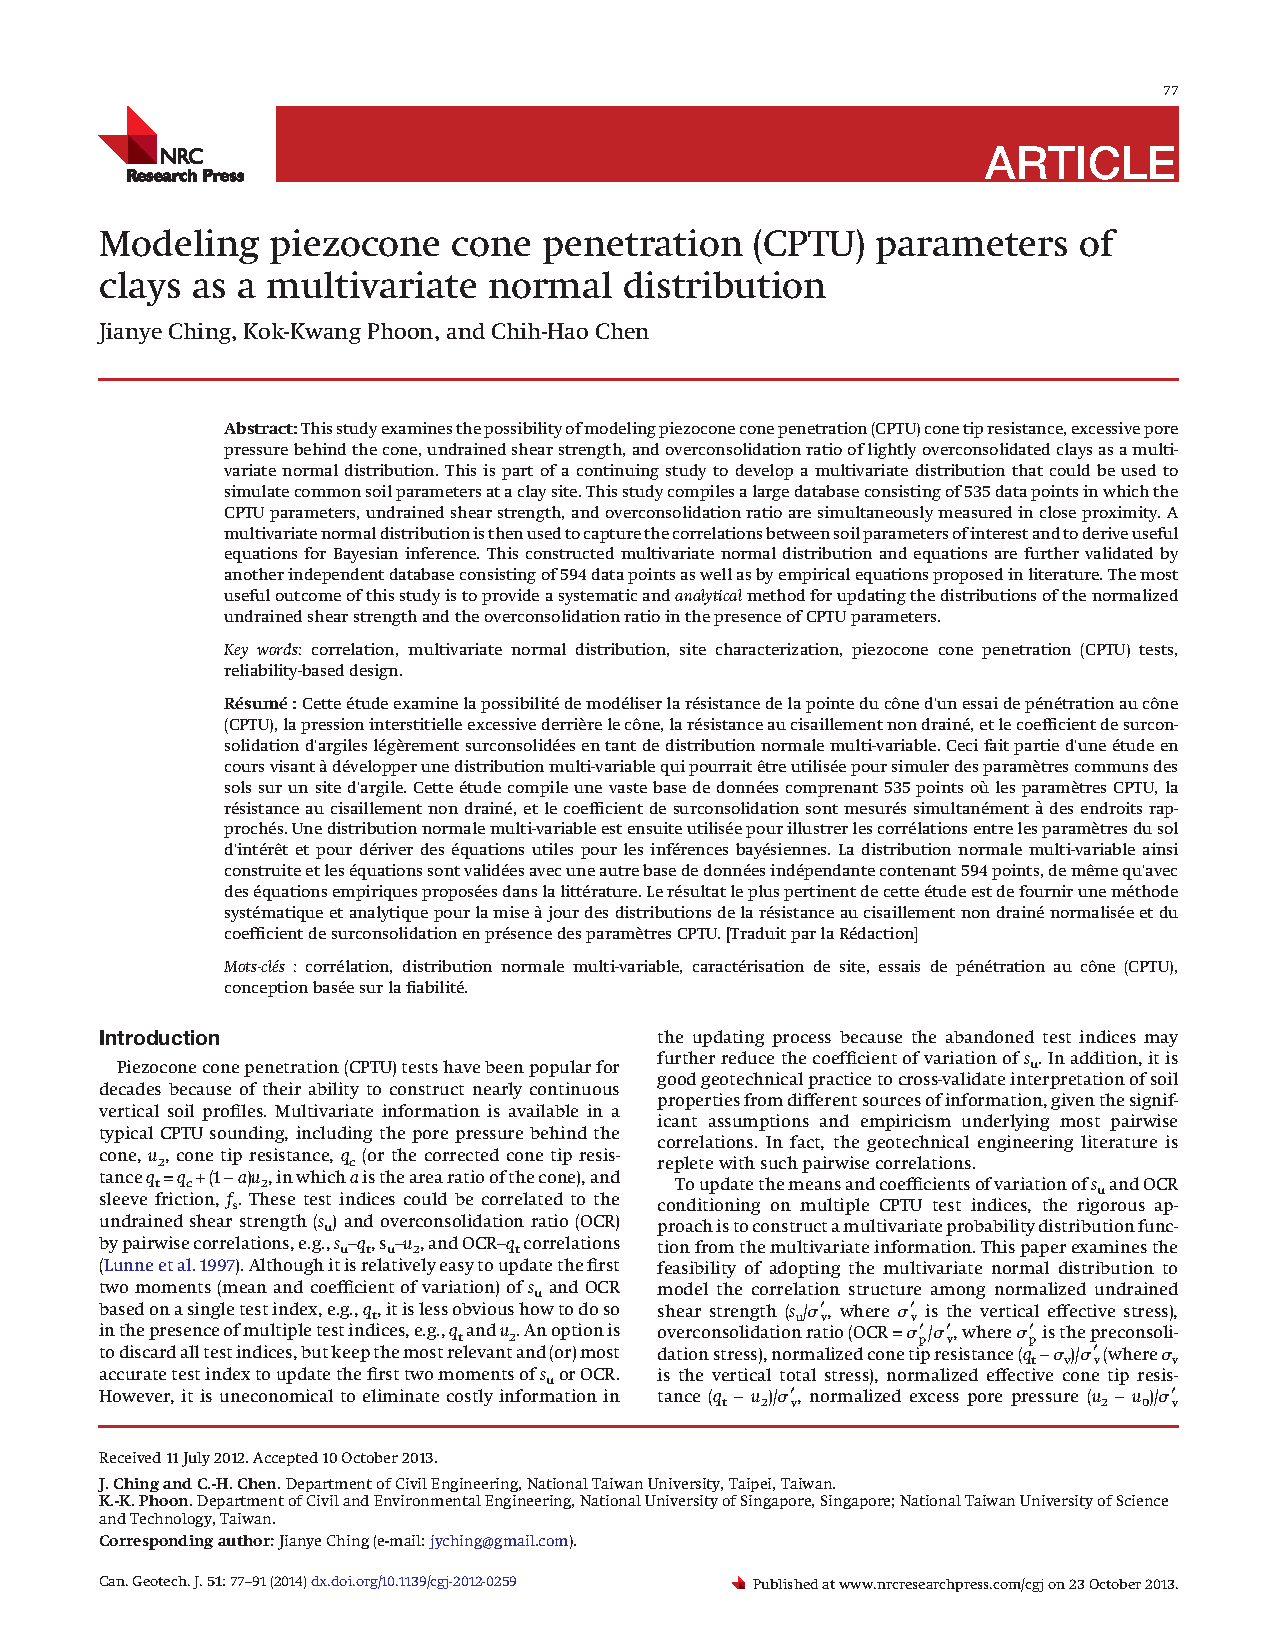
\includepdf[pages=1-last]{PDFs/Ching2014-Modeling piezocone cone penetration (CPTU) parameters of clays as a multivariate normal distribution.pdf}
	\label{bib:3}
	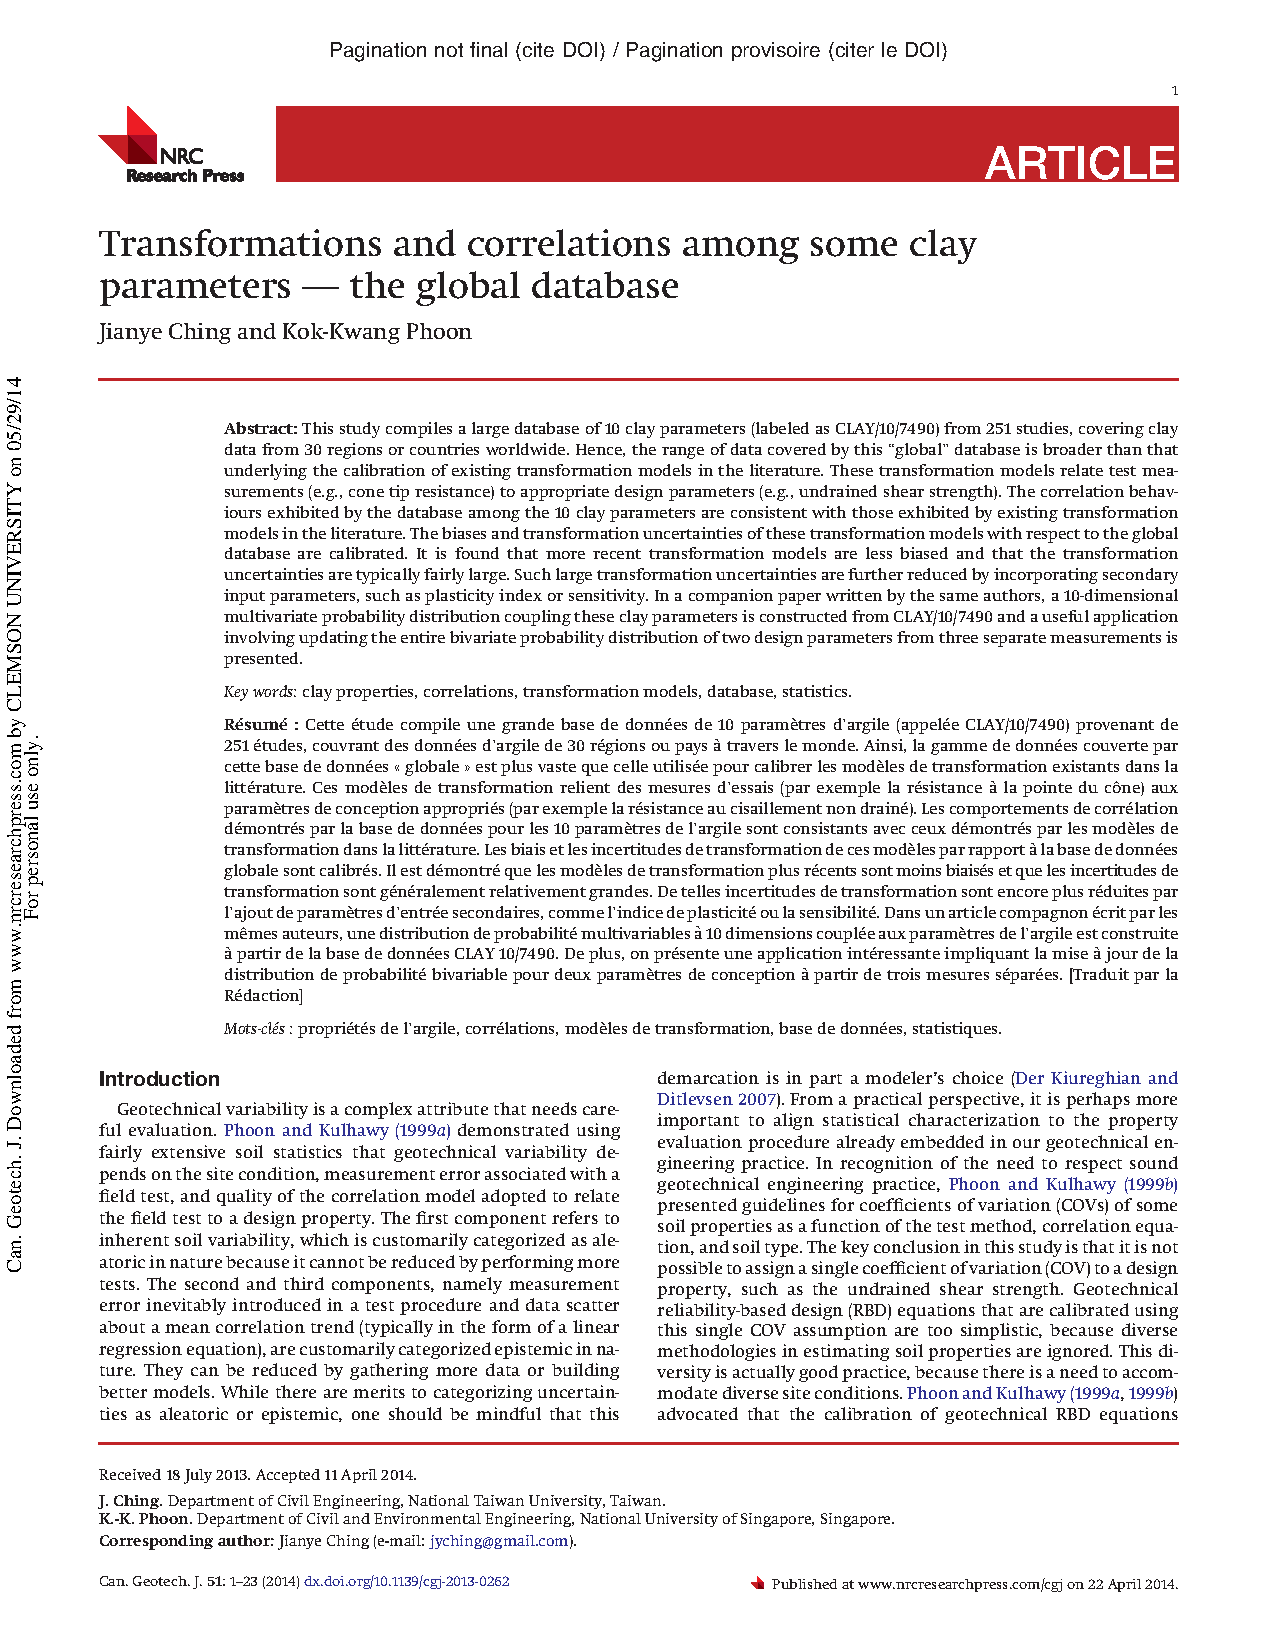
\includepdf[pages=1-last]{PDFs/Ching2014-Transformations and correlations among some clay parameters - the global database.pdf}
	\label{bib:4}
	\includepdf[pages=1-last]{PDFs/Ching2014-Correlations among some clay parameters - the multivariate distribution.pdf}
	\label{bib:5}
	\includepdf[pages=1-last]{PDFs/D’Ignazio2016-Correlations for undrained shear strength of Finnish soft clays.pdf}
	\label{bib:6}
	\includepdf[pages=1-last]{PDFs/D’Ignazio2016-Correlations for undrained shear strength of Finnish soft clays.pdf}
	\label{bib:7}
	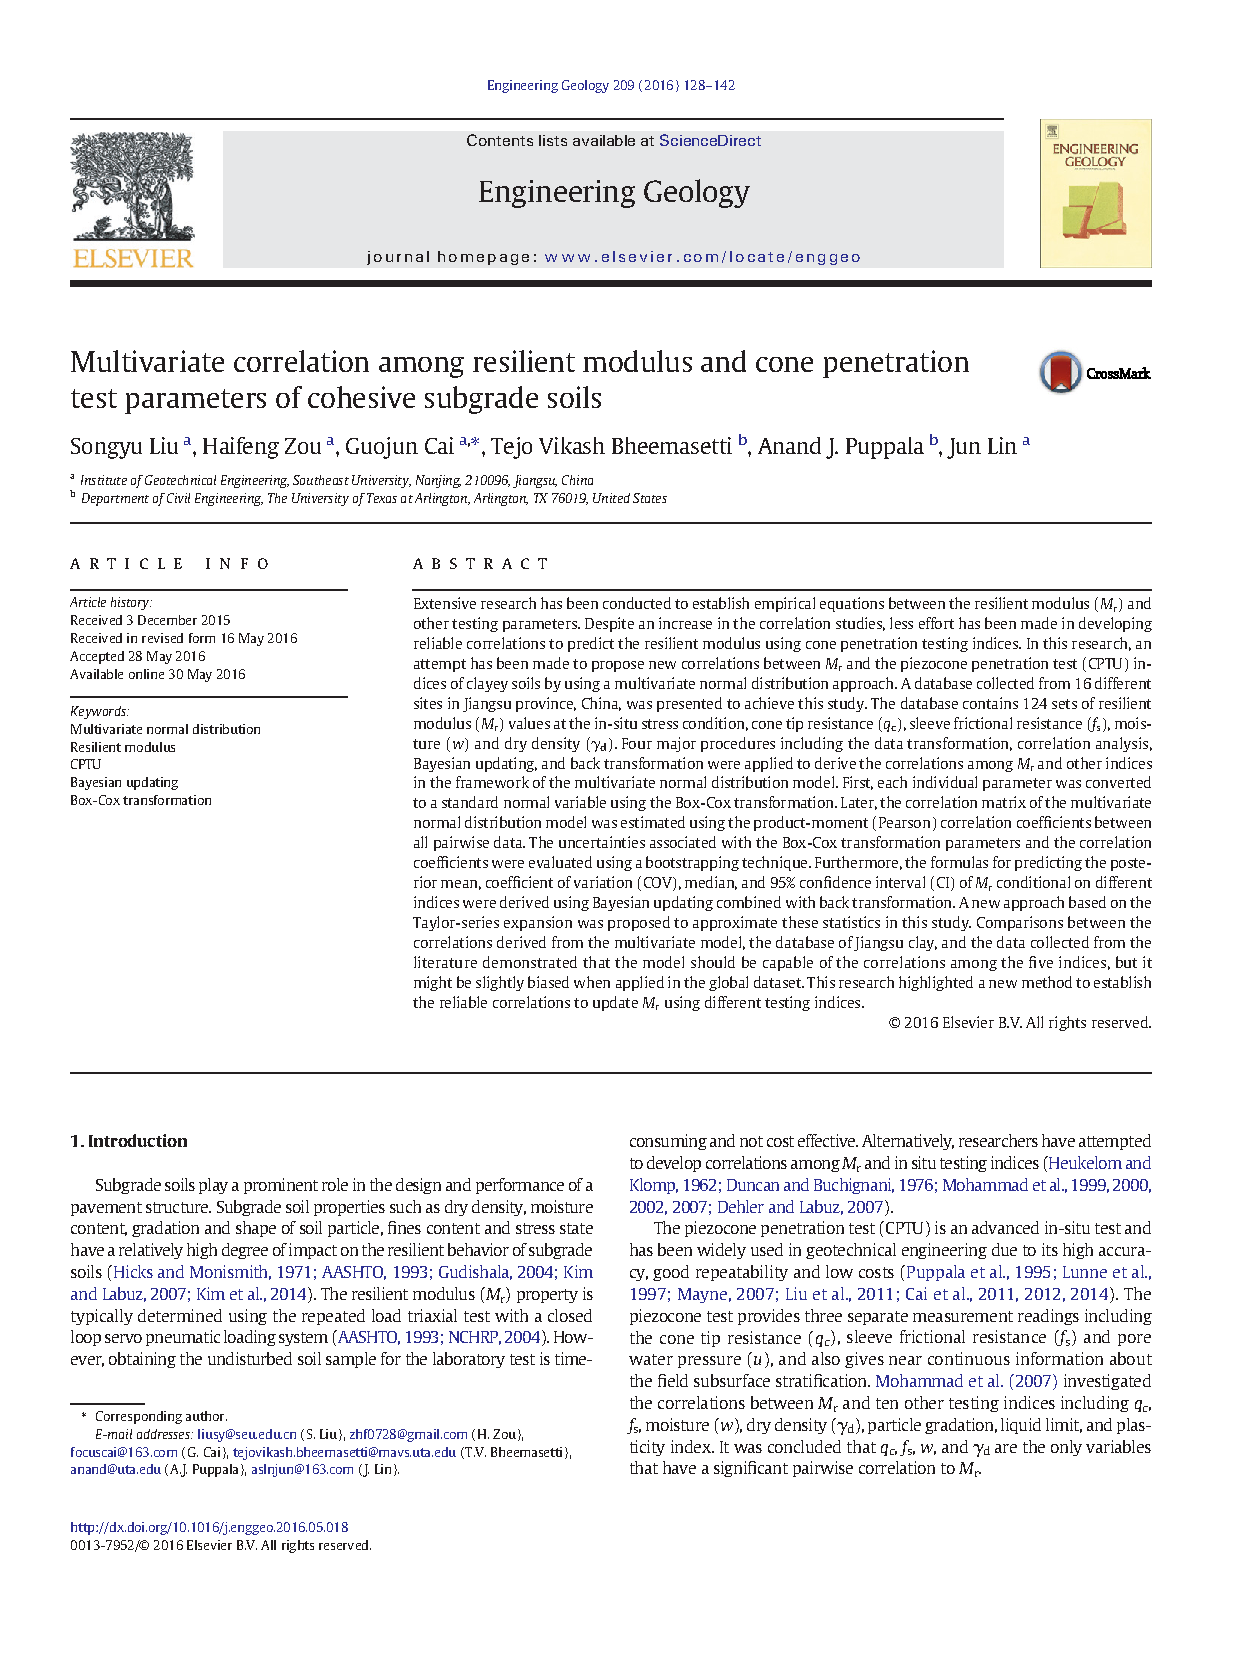
\includepdf[pages=1-last]{PDFs/Liu2016-Multivariate correlation among resilient modulus and cone penetration test parameters of cohesive subgrade soils.pdf}
	\label{bib:8}
	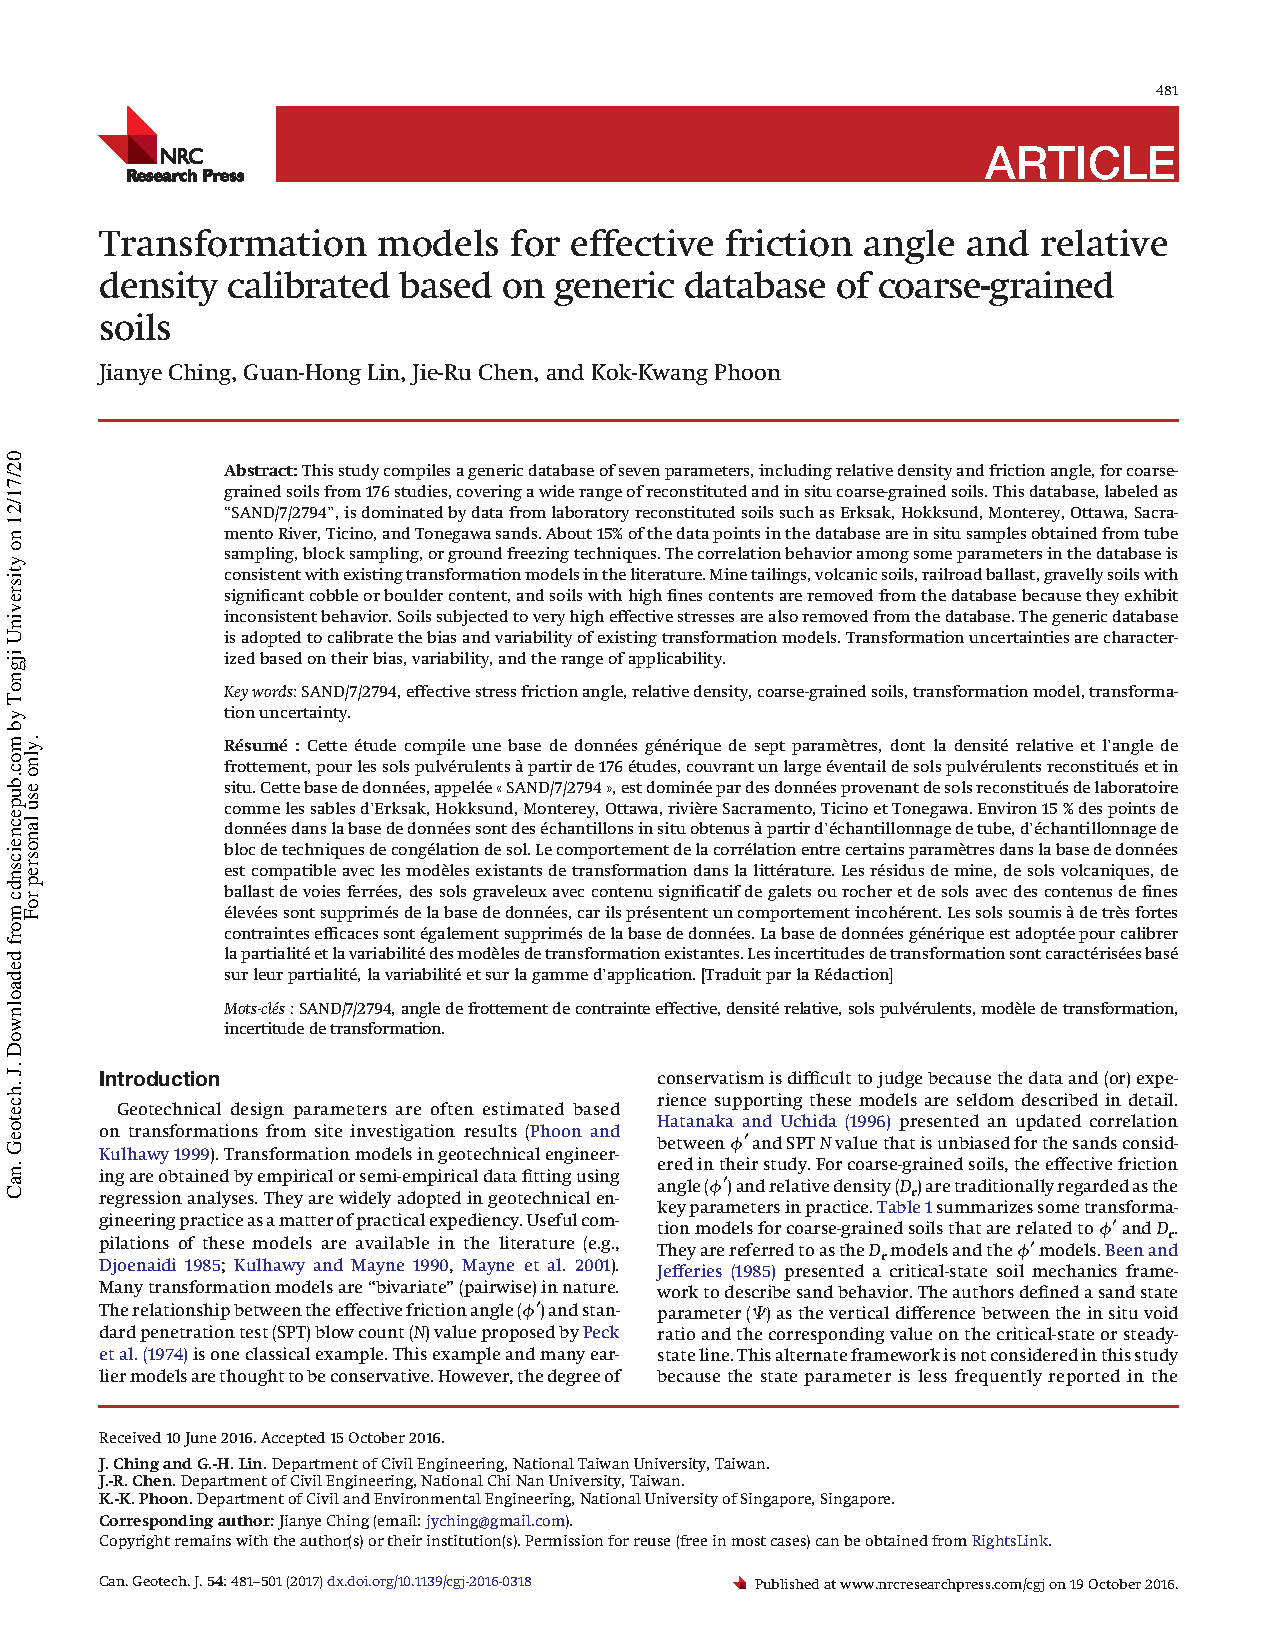
\includepdf[pages=1-last]{PDFs/Ching2017-Transformation models for effective friction angle and relative density calibrated based on generic database of coarse-grained soils.pdf}
	\label{bib:9}
	\includepdf[pages=1-last]{PDFs/Ching2018-Generic transformation models for some intact rock properties.pdf}
	\label{bib:10}
	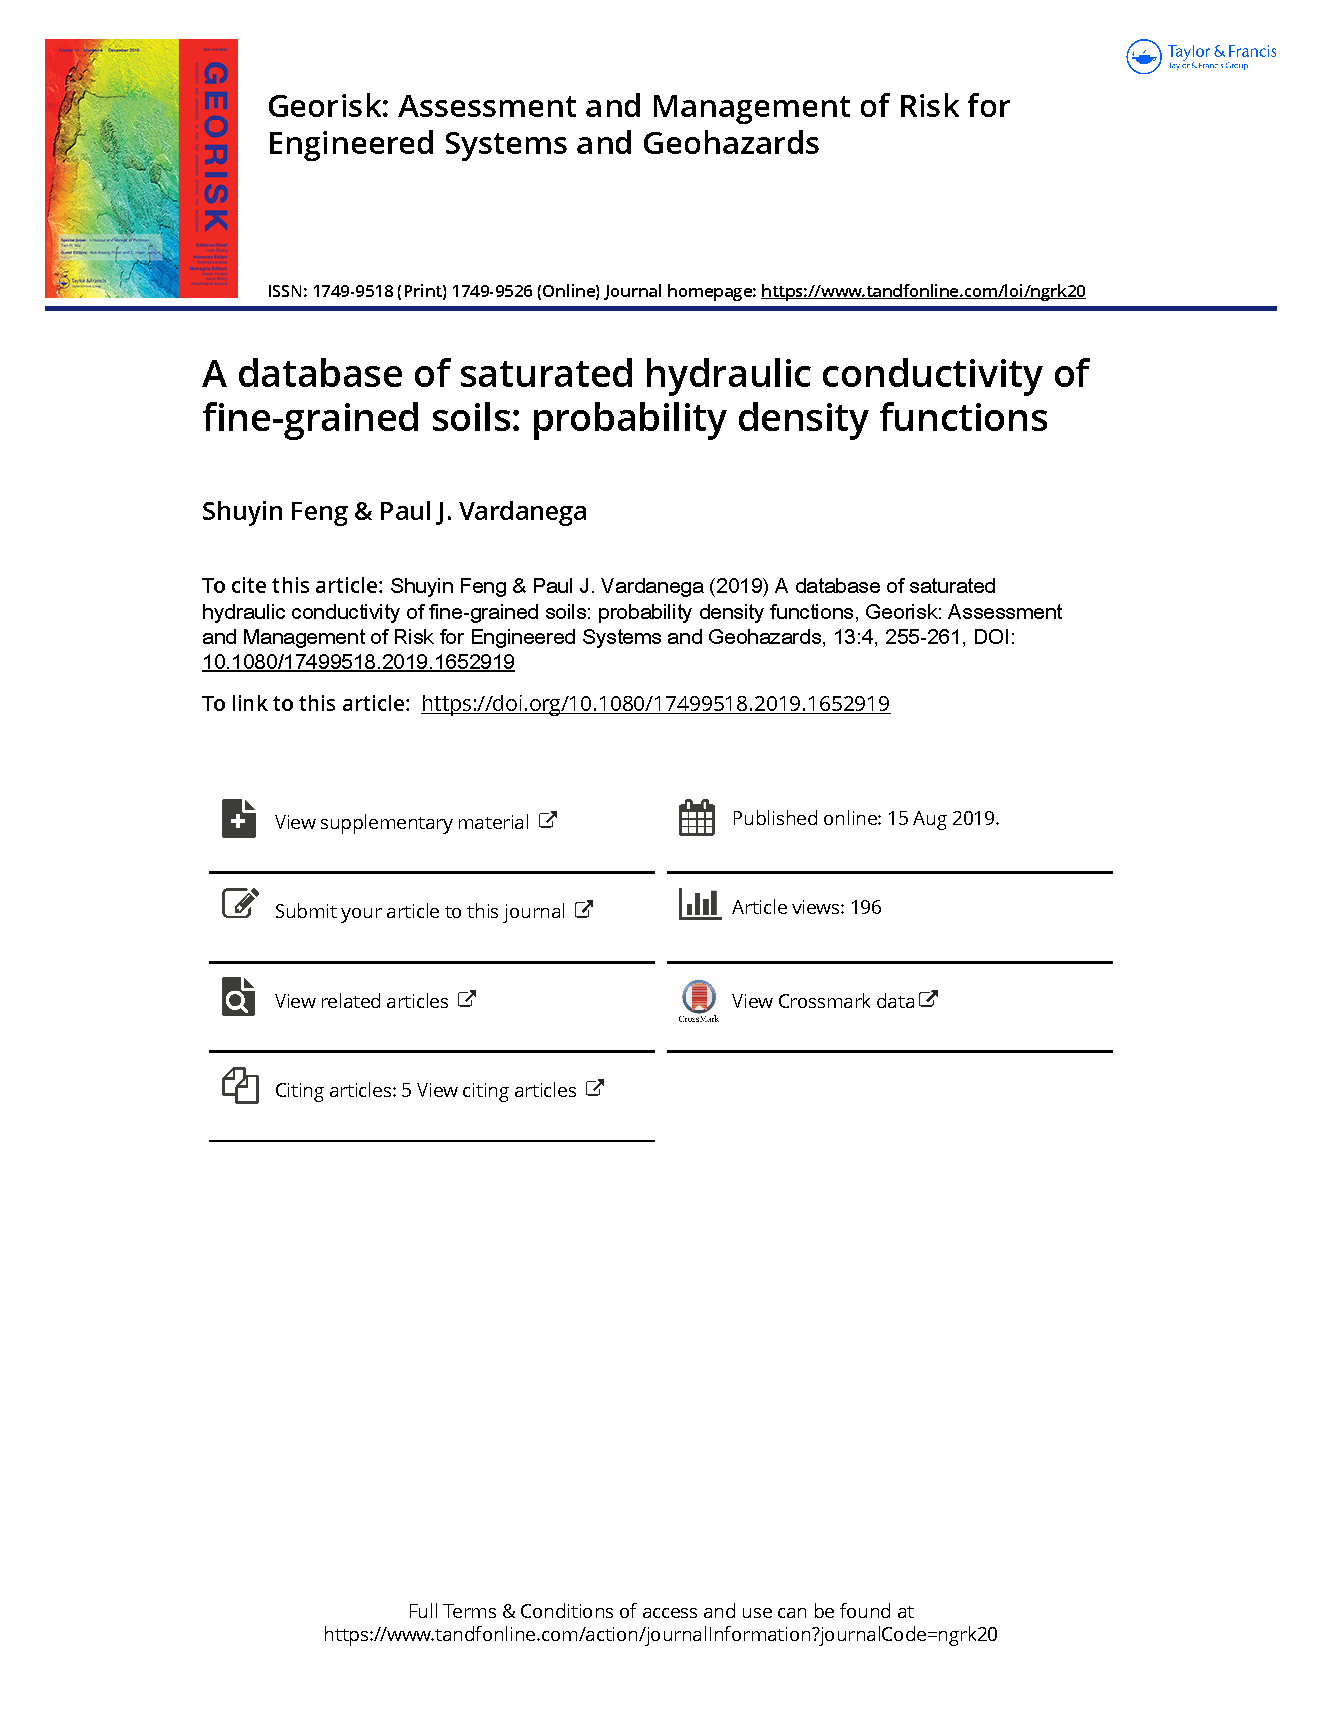
\includepdf[pages=1-last]{PDFs/Feng2019a-A database of saturated hydraulic conductivity of fine-grained soils- probability density functions.pdf}
	\label{bib:11}
	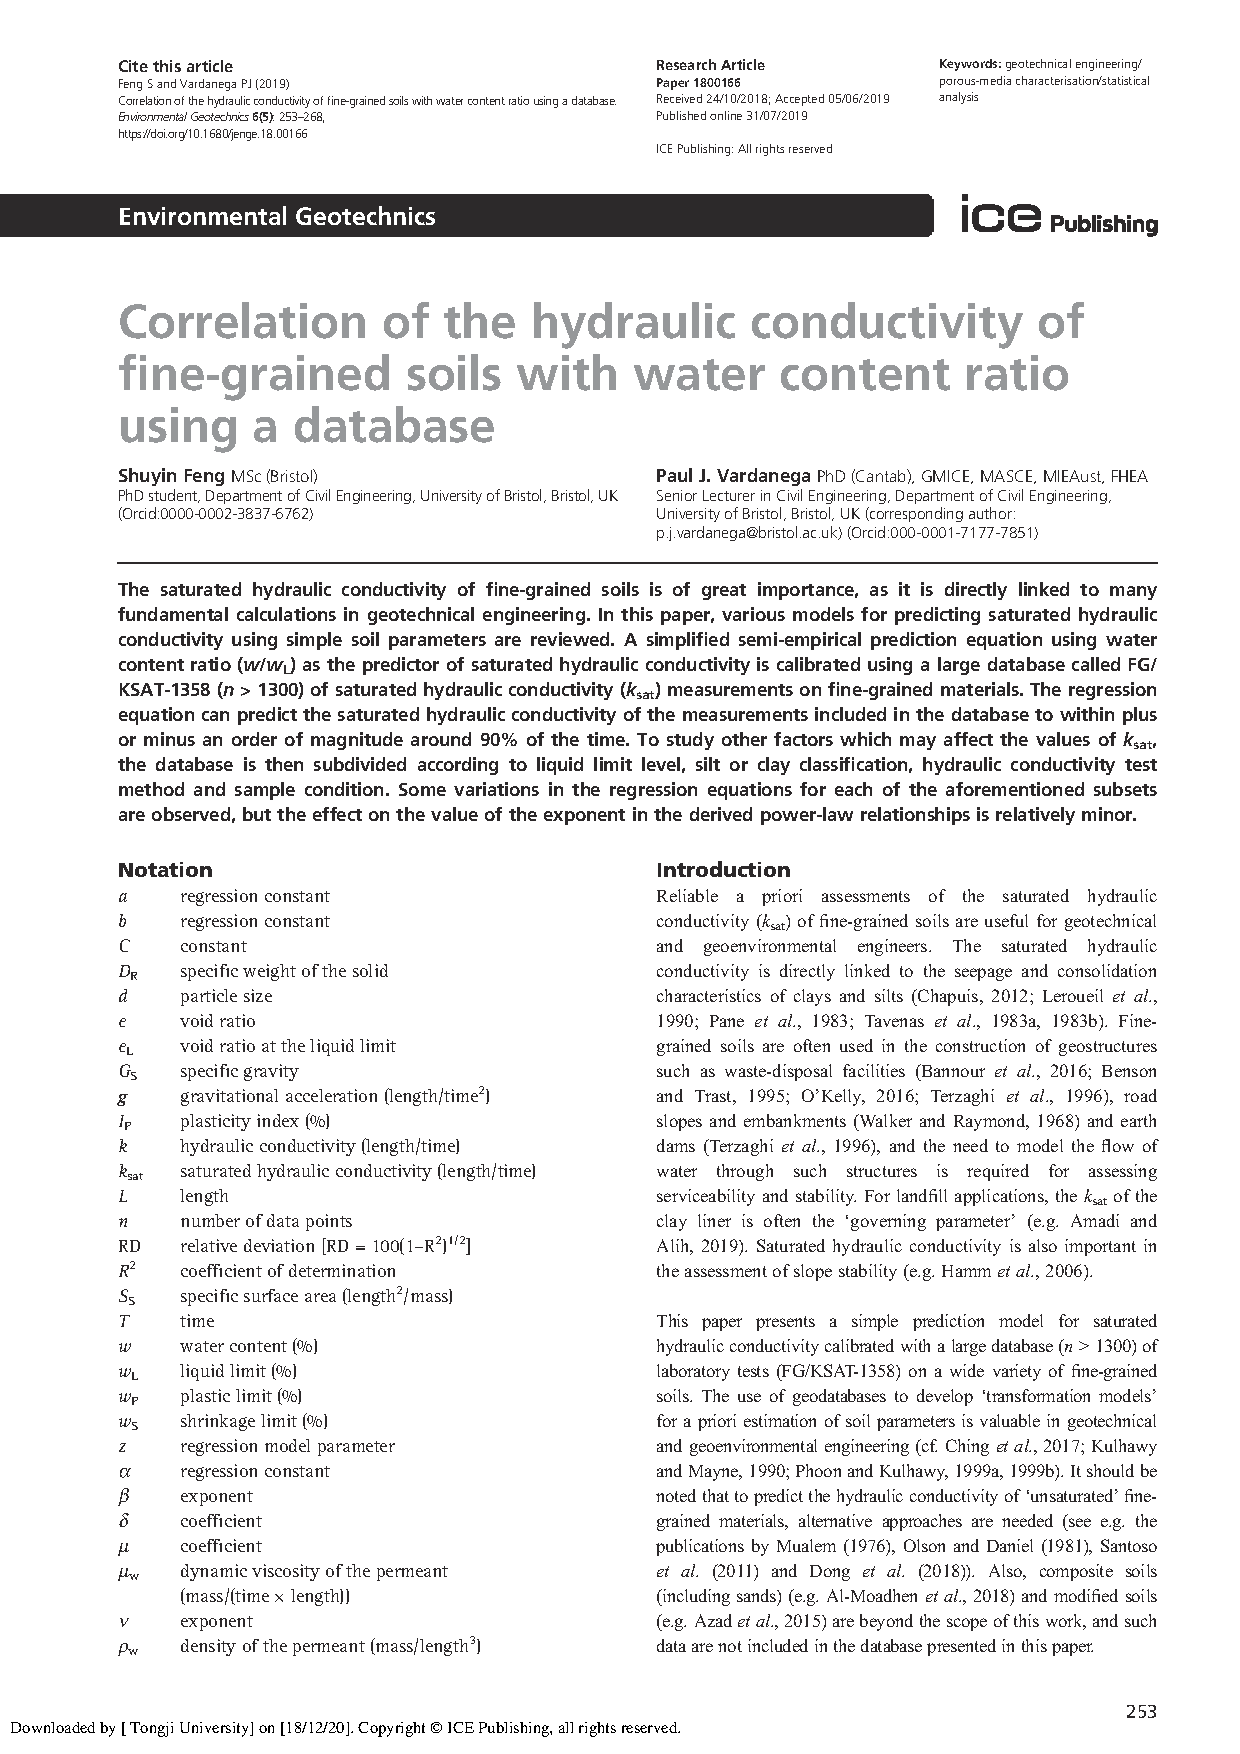
\includepdf[pages=1-last]{PDFs/Feng2019b-Full AccessCorrelation of the hydraulic conductivity of fine-grained soils with water content ratio using a database.pdf}
	\label{bib:12}
	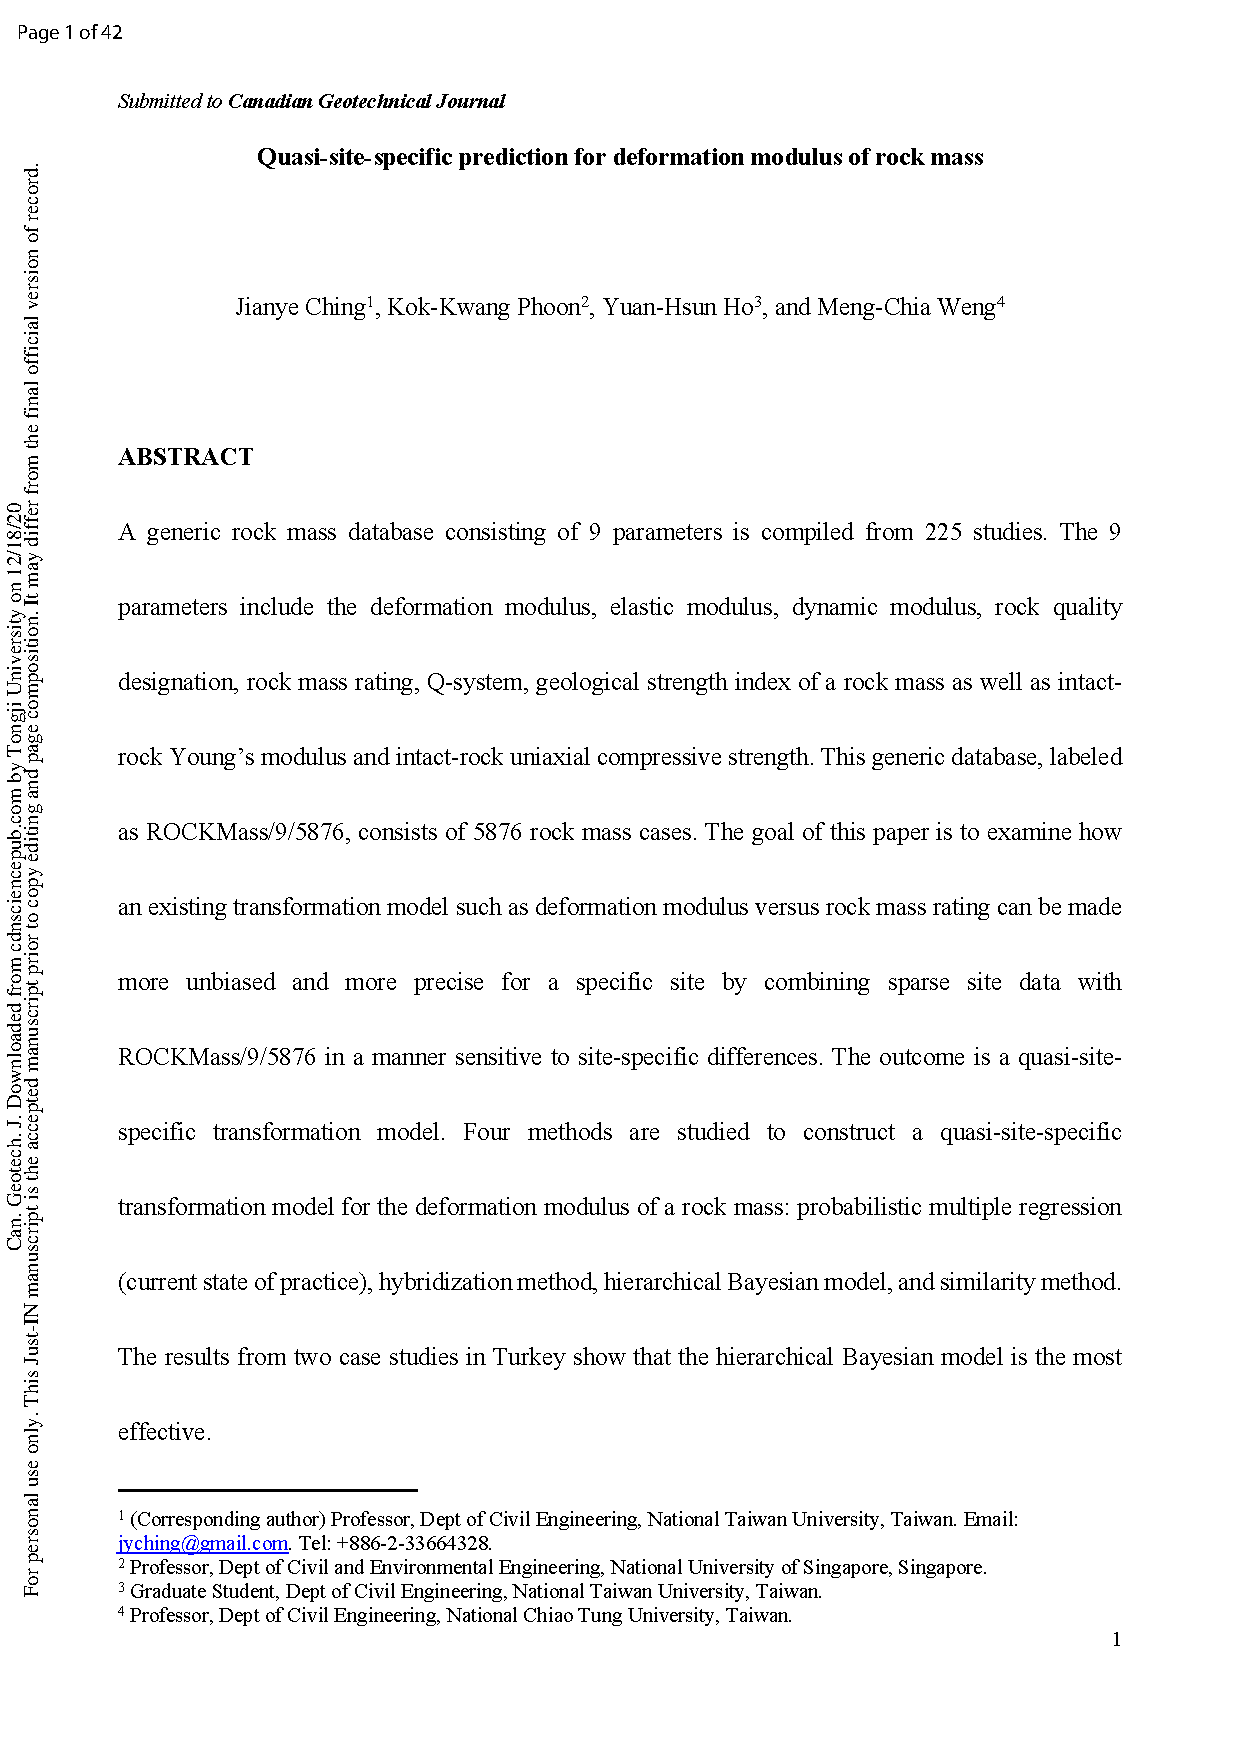
\includepdf[pages=1-last]{PDFs/Ching2020-Quasi-site-specific prediction for deformation modulus of rock mass.pdf}
	\label{bib:13}
	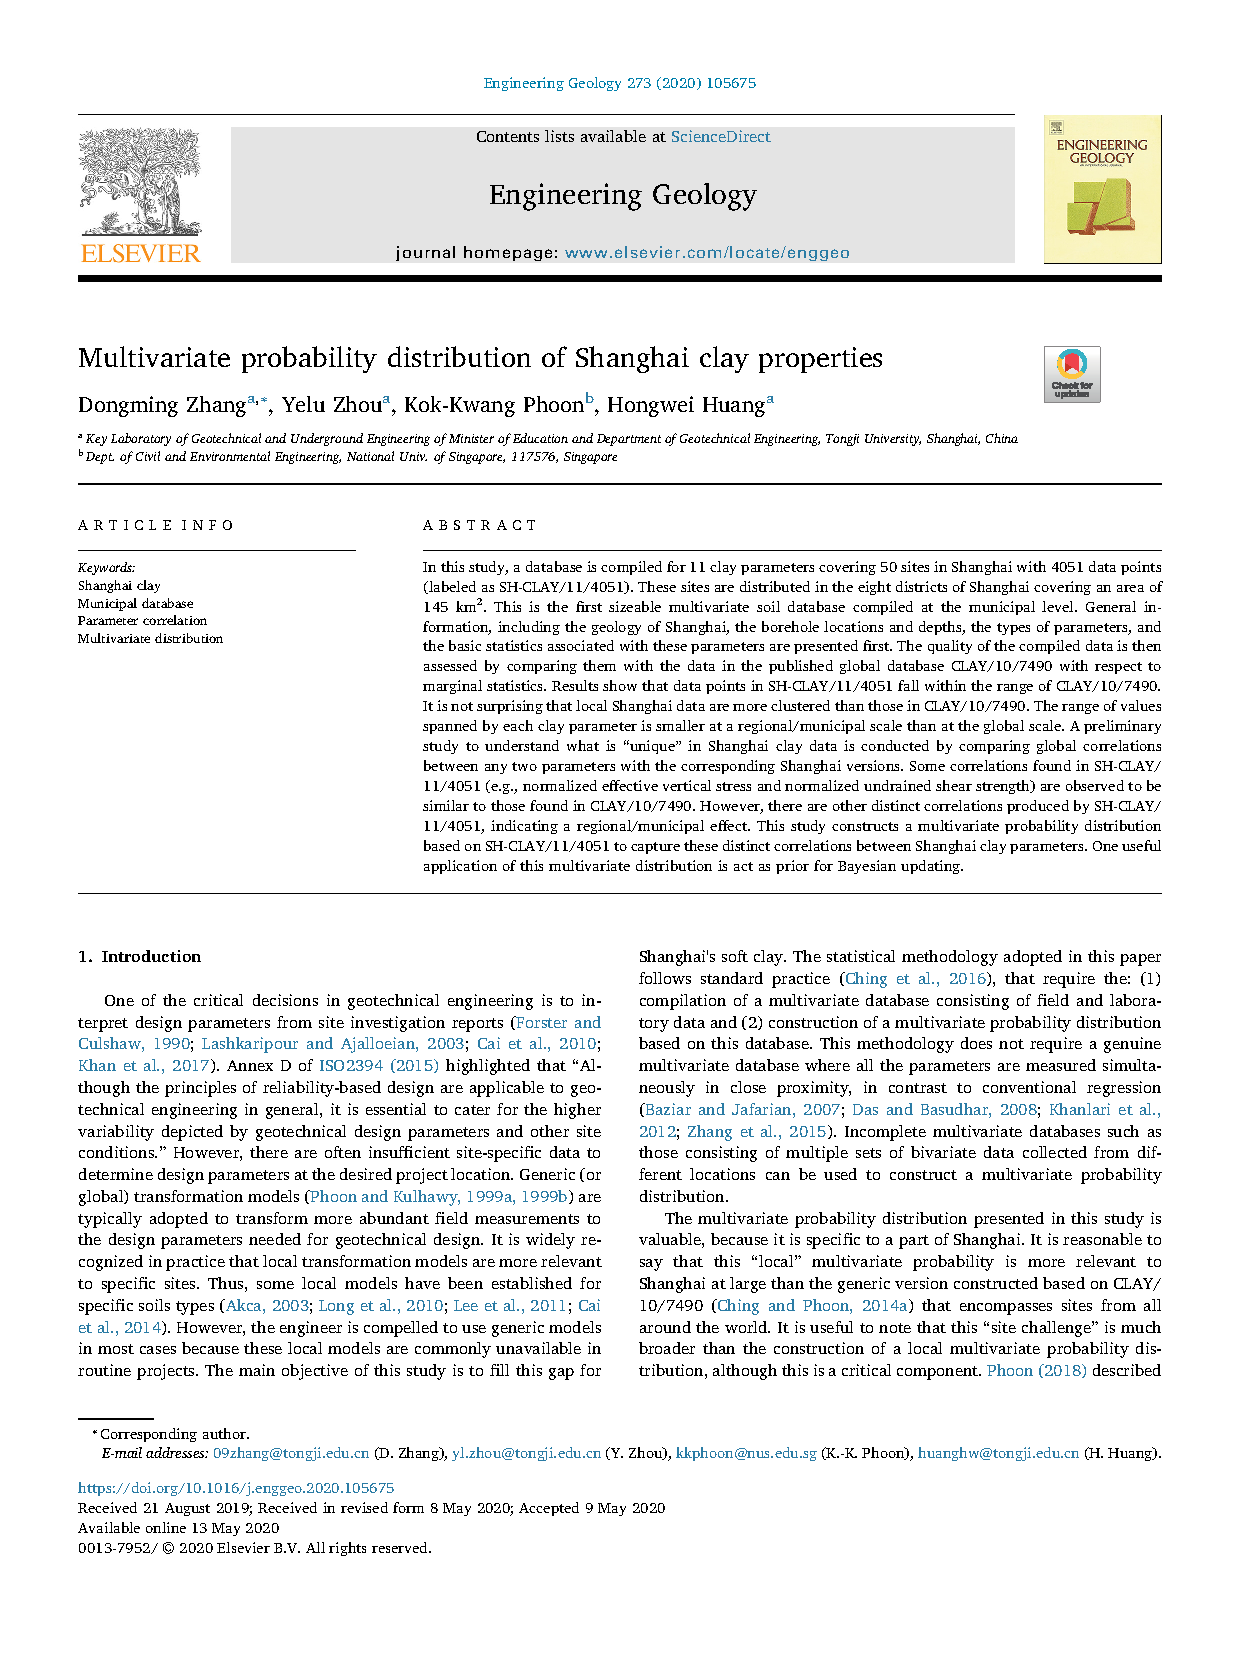
\includepdf[pages=1-last]{PDFs/Zhang dongming 2020-Multivariate probability distribution of shanghai clay properties.pdf}
	\label{bib:14}
	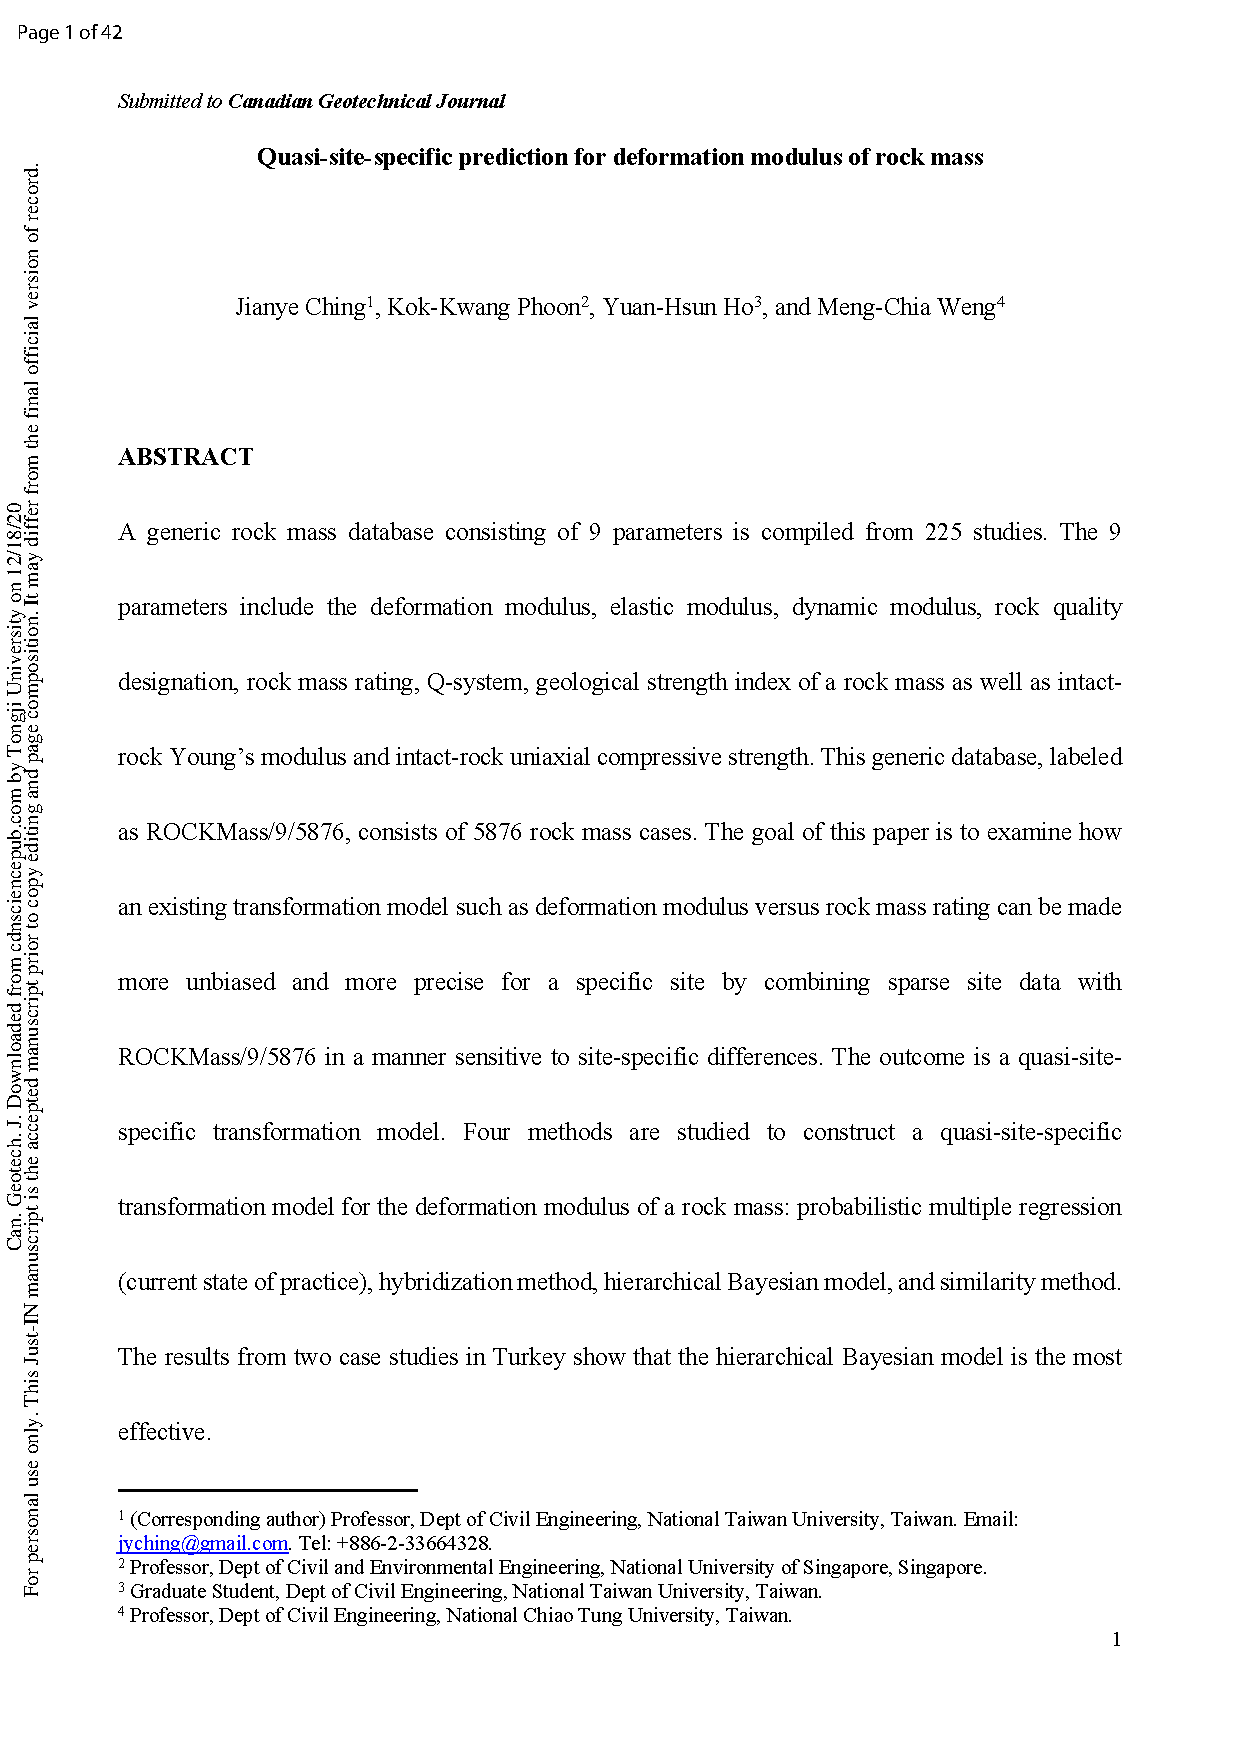
\includepdf[pages=1-last]{PDFs/Ching2020-Quasi-site-specific prediction for deformation modulus of rock mass.pdf}
	\label{bib:15}
	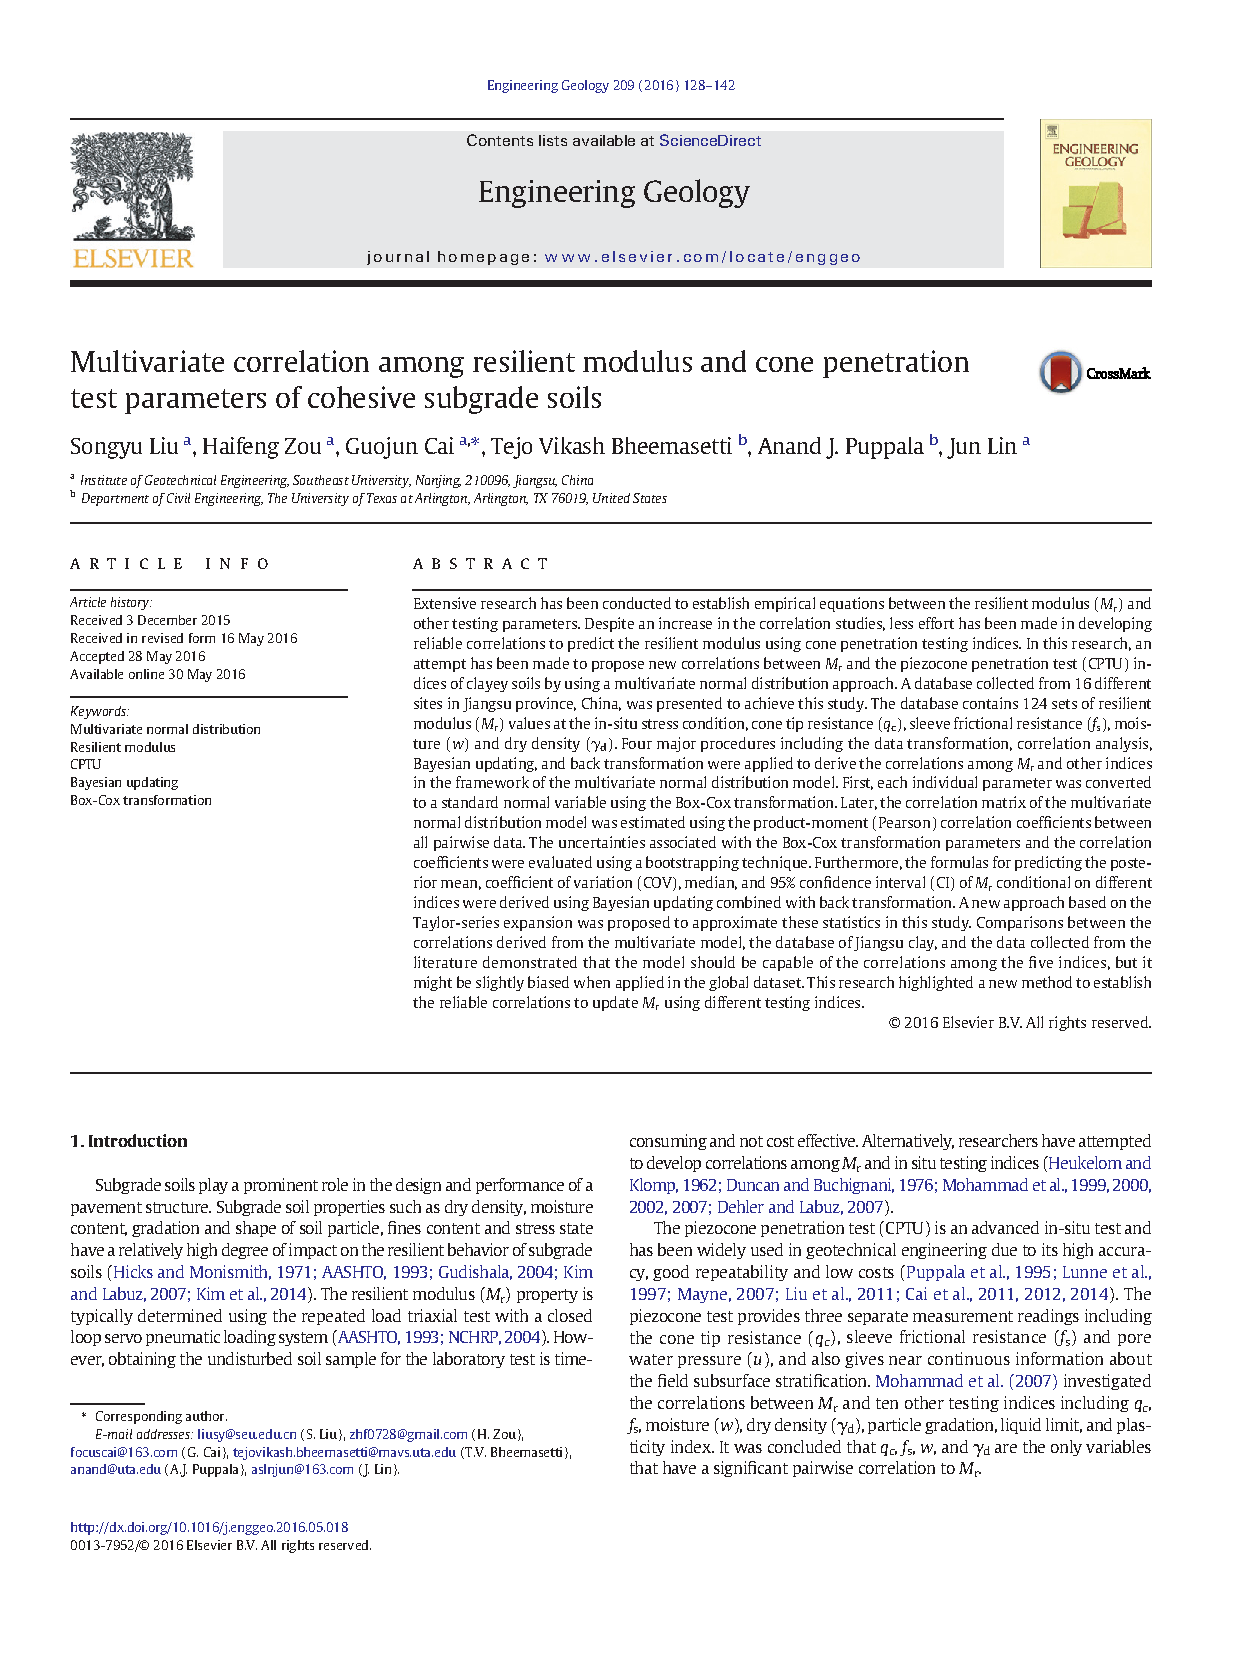
\includepdf[pages=1-last]{PDFs/Liu2016-Multivariate correlation among resilient modulus and cone penetration test parameters of cohesive subgrade soils.pdf}

\end{document}